\chapter{Cadre général du projet}

\noindent\textbf{Plan du chapitre}
\begin{enumerate}[nosep]
  \item Introduction
  \item Présentation de l'organisme d'accueil
  \item Analyse de l'existant et critique des solutions du marché
  \item Problématique
  \item Solution proposée~: la plateforme GerAI
  \item Feuille de route du projet
  \item Méthodologie de développement~: Scrum
  \item Conclusion
\end{enumerate}

% ─────────────────────────────────────────────────────────────
\section{Introduction}
% ─────────────────────────────────────────────────────────────

Toute organisation dont l'actif principal est humain souffre, au-delà d'un certain
seuil d'effectifs, d'une inadéquation structurelle entre la complexité de ses
processus RH et la rudimentarité des outils qu'elle utilise pour les gérer. Arabsoft,
entreprise tunisienne de développement logiciel sur mesure, illustre parfaitement
cette tension~: ses équipes techniques produisent des applications de gestion
sophistiquées pour leurs clients, tandis que leurs propres processus RH internes
reposent encore sur des échanges de mails et des tableurs partagés. Ce chapitre
présente l'entreprise, analyse l'existant et ses limites, formule la problématique
centrale, décrit la solution \textbf{GerAI} et expose la méthodologie Scrum retenue.

% ─────────────────────────────────────────────────────────────
\section{Présentation de l'organisme d'accueil}
% ─────────────────────────────────────────────────────────────

\subsection{Historique et domaine d'activité}

Arabsoft est une société tunisienne spécialisée dans l'édition de logiciels sur
mesure et l'intégration de systèmes d'information. Fondée avec pour vocation
d'accompagner les entreprises locales dans leur transformation numérique, elle
intervient sur l'ensemble du cycle de vie des projets informatiques~: de l'analyse
fonctionnelle à la mise en production, en passant par la conception, le développement
et la formation des utilisateurs finaux. Son catalogue technique couvre le
développement \textit{full-stack} Java/Angular, la \textit{business intelligence}
Oracle, les applications mobiles cross-platform, et la maintenance évolutive de
systèmes patrimoniaux.

Au fil des années, Arabsoft s'est imposée comme partenaire de confiance d'entreprises
industrielles, financières et administratives qui lui confient des missions à fort
enjeu métier. Cette position lui a permis de développer une expertise approfondie
des processus de gestion, dont elle exploite aujourd'hui les enseignements pour
digitaliser ses propres opérations internes~--- à commencer par la gestion de ses
ressources humaines, longtemps délaissée au profit du business client.

\subsection{Fiche d'identité}

\begin{table}[H]
\centering
\caption{Fiche d'identité d'Arabsoft}
\label{tab:fiche}
\begin{tabularx}{\textwidth}{|l|L|}
\hline
\rowcolor{headerblue!25}\textbf{Champ} & \textbf{Valeur} \\\hline
\rowcolor{rowgray}Raison sociale & Arabsoft \\\hline
Forme juridique & Société à responsabilité limitée (SARL) \\\hline
\rowcolor{rowgray}Secteur d'activité & Édition de logiciels sur mesure, intégration de systèmes d'information \\\hline
Domaines techniques & Java/Spring Boot, Angular, Oracle Database, BI, mobilité \\\hline
\rowcolor{rowgray}Marchés servis & Finance, industrie, administration publique, services \\\hline
Types de missions & Développement sur mesure, intégration SI, maintenance évolutive \\\hline
\rowcolor{rowgray}Stack principale & Java 21, TypeScript, Oracle 23ai, Docker, Keycloak \\\hline
Méthodologies & Scrum (projets internes), cycle en V (projets à périmètre figé) \\\hline
\end{tabularx}
\end{table}

\subsection{Organigramme}

La structure organisationnelle d'Arabsoft s'articule autour de trois pôles
fonctionnels~: un pôle technique regroupant les développeurs et architectes~;
un pôle commercial couvrant l'avant-vente et la relation client~; et un pôle
support assurant la maintenance et la qualité. Chaque pôle dispose d'un
responsable rattaché à la direction générale.

\begin{figure}[H]
\centering
\begin{tikzpicture}[
  dg/.style={draw, rounded corners=5pt, fill=headerblue!40, minimum width=4.5cm,
             minimum height=0.85cm, font=\small\bfseries, align=center},
  pole/.style={draw, rounded corners=4pt, fill=umlblue!35, minimum width=3.2cm,
               minimum height=0.8cm, font=\small, align=center},
  equipe/.style={draw, rounded corners=3pt, fill=umlgray, minimum width=2.8cm,
                 minimum height=0.7cm, font=\scriptsize, align=center},
  arr/.style={->, >=stealth, thick}
]
  \node[dg] (dg) at (5.5, 5.5) {Direction Générale};
  \node[pole] (tech) at (1.2,  3.5) {Pôle Technique};
  \node[pole] (com)  at (5.5,  3.5) {Pôle Commercial};
  \node[pole] (sup)  at (9.8,  3.5) {Pôle Support};

  \node[equipe] (dev)  at (0,   1.5) {Développeurs};
  \node[equipe] (arc)  at (3.0, 1.5) {Architectes};
  \node[equipe] (av)   at (4.4, 1.5) {Avant-vente};
  \node[equipe] (rc)   at (7.0, 1.5) {Relation client};
  \node[equipe] (mnt)  at (8.6, 1.5) {Maintenance};
  \node[equipe] (qa)   at (11.4,1.5) {Tests / QA};

  \draw[arr] (dg) -- (tech);
  \draw[arr] (dg) -- (com);
  \draw[arr] (dg) -- (sup);
  \draw[arr] (tech) -- (dev);
  \draw[arr] (tech) -- (arc);
  \draw[arr] (com)  -- (av);
  \draw[arr] (com)  -- (rc);
  \draw[arr] (sup)  -- (mnt);
  \draw[arr] (sup)  -- (qa);
\end{tikzpicture}
\caption{Organigramme d'Arabsoft}
\label{fig:orga}
\end{figure}

\subsection{Orientations stratégiques}

La direction générale d'Arabsoft a défini trois axes prioritaires~:
\begin{enumerate}
  \item \textbf{Internalisation des outils de pilotage}~: se doter d'une
        plateforme interne pour chaque processus métier critique, réduisant
        la dépendance aux outils génériques et servant de vitrine technique
        pour les clients potentiels.
  \item \textbf{Capitalisation sur la donnée RH}~: constituer un historique
        structuré permettant des analyses décisionnelles~--- taux d'absentéisme,
        évolution des compétences, anticipation des risques de départ~--- jusqu'ici
        impossibles faute d'un référentiel centralisé.
  \item \textbf{Modernisation architecturale}~: migrer les projets internes
        vers une architecture microservices pour démontrer la maîtrise de ces
        technologies et en bénéficier opérationnellement (scalabilité, isolation).
\end{enumerate}

% ─────────────────────────────────────────────────────────────
\section{Analyse de l'existant et critique des solutions du marché}
% ─────────────────────────────────────────────────────────────

\subsection{Description du système existant}

Avant ce projet, la gestion des ressources humaines chez Arabsoft reposait sur
un empilement d'outils génériques~:

\begin{itemize}
  \item \textbf{Congés et absences}~: demandes soumises et approuvées par e-mail
        entre l'employé, son chef et le département RH. Aucune référence de suivi,
        aucun contrôle automatique du solde disponible, aucune alerte en cas
        de chevauchement.
  \item \textbf{Formations}~: planification dans des tableurs Excel partagés via
        réseau. Doublons d'inscription non détectés, budget formation non suivi.
  \item \textbf{Prêts au personnel}~: circuit entièrement informel~; montant,
        durée et décision de la commission ne sont pas consignés systématiquement.
  \item \textbf{Documents administratifs}~: demandes d'attestations ou de
        bulletins de paie adressées par messagerie interne, sans accusé de
        traitement ni délai garanti.
  \item \textbf{Projets et tâches}~: suivi par réunions hebdomadaires et post-its~;
        l'avancement est estimé subjectivement, jamais calculé.
\end{itemize}

\begin{table}[H]
\centering
\caption{Dysfonctionnements du système existant et impacts mesurés}
\label{tab:critique}
\begin{tabularx}{\textwidth}{|l|L|L|}
\hline
\rowcolor{headerblue!25}\textbf{Domaine} & \textbf{Dysfonctionnement} & \textbf{Impact} \\\hline
\rowcolor{rowgray}
Congés & Approbation par e-mail non tracée &
  Litiges sur soldes~; incohérences entre RH et employés \\\hline
Formations & Planification manuelle (tableur partagé) &
  Dépassements budgétaires~; doublons d'inscription \\\hline
\rowcolor{rowgray}
Prêts & Circuit informel, décisions non documentées &
  Risque juridique~; historique inexploitable par la comptabilité \\\hline
Documents & Demandes par messagerie interne &
  Délais non maîtrisés~; relances manuelles répétées \\\hline
\rowcolor{rowgray}
Projets/Tâches & Aucun outil centralisé &
  Avancement non mesurable~; retards non anticipés \\\hline
Reporting RH & Extraction manuelle multi-sources &
  Indicateurs obsolètes~; analytique prédictive impossible \\\hline
\end{tabularx}
\end{table}

\subsection{Analyse des solutions SIRH existantes}

Quatre familles de solutions ont été examinées avant de retenir le développement
sur mesure~:

\begin{table}[H]
\centering
\caption{Comparaison des solutions SIRH selon les critères d'Arabsoft}
\label{tab:sirh}
\begin{tabularx}{\textwidth}{|l|C|C|C|C|}
\hline
\rowcolor{headerblue!25}\textbf{Critère} &
  \shortstack{\textbf{SAP}\\\textbf{Success}\\\textbf{Factors}} &
  \shortstack{\textbf{Oracle}\\\textbf{HCM}\\\textbf{Cloud}} &
  \shortstack{\textbf{Sage}\\\textbf{RH}} &
  \shortstack{\textbf{Orange}\\\textbf{HRM}} \\\hline
\rowcolor{rowgray}
Coût de licence & \ding{55} Élevé & \ding{55} Élevé & Moyen & Gratuit \\\hline
Déploiement on-premise & Non & Partiel & Oui & Oui \\\hline
\rowcolor{rowgray}
Personnalisation workflow & Faible & Faible & Moyenne & Faible \\\hline
API REST complète & Partielle & Partielle & Limitée & Limitée \\\hline
\rowcolor{rowgray}
Analytique prédictive & Module \$\$ & Module \$\$ & Non & Non \\\hline
Intégration Keycloak & Non & Non & Non & Non \\\hline
\rowcolor{rowgray}
Maîtrise du code source & Non & Non & Non & Partielle \\\hline
Adapté au droit tunisien & Non & Non & Partielle & Non \\\hline
\end{tabularx}
\end{table}

\subsubsection*{Limitations techniques}

Les plateformes SaaS (SAP, Oracle HCM) n'exposent que les APIs prévues par
l'éditeur. L'intégration d'un bus d'événements Kafka pour la notification
asynchrone, ou d'un serveur Keycloak pour une authentification centralisée
inter-applications, est impossible sans développements propriétaires facturés
au forfait et sans garantie de support à long terme. L'absence d'accès au
code source interdit toute correction d'un comportement non conforme aux règles
de gestion spécifiques à Arabsoft.

\subsubsection*{Limitations de scalabilité}

Le modèle de tarification à l'utilisateur implique un TCO directement
proportionnel à la croissance des effectifs~: chaque recrutement augmente le
coût de la plateforme. Par ailleurs, l'architecture monolithique de ces solutions
ne permet pas de mettre à l'échelle un seul module (par exemple l'analytique ou
la messagerie) sans toucher à l'ensemble de l'infrastructure.

\subsubsection*{Limitations de personnalisation}

Le circuit de validation des prêts d'Arabsoft~--- commission de crédit, vote
par seuil, routage conditionnel selon l'indicateur \texttt{NEEDS\_COMMISSION}~---
ne peut pas être modélisé dans ces outils sans développement complémentaire.
Les workflows sont configurables dans des bornes fixées par l'éditeur~: ajouter
une étape ou créer une logique de routage conditionnelle nécessite un contrat
de personnalisation distinct.

\subsubsection*{Limitations du suivi analytique}

Les modules analytiques des SIRH commerciaux sont soit absents des offres de
base, soit disponibles comme extensions payantes. Aucun d'eux n'intègre un module
de prédiction de l'attrition adapté aux données internes d'Arabsoft~: calculer
un score de risque de départ directement depuis les requêtes Oracle sur les tables
\texttt{EMPLOYEES}, \texttt{LEAVE\_REQUESTS} et \texttt{PROJECT\_MEMBERS} n'est
pas une fonctionnalité proposée par ces éditeurs.

% ─────────────────────────────────────────────────────────────
\section{Problématique}
% ─────────────────────────────────────────────────────────────

\begin{tcolorbox}[colback=blue!5, colframe=headerblue,
                  title=\textbf{Problématique centrale}]
Comment concevoir et livrer une plateforme GRH centralisée qui~:
automatise cinq types de demandes RH avec un circuit de validation hiérarchique
paramétrable~; gère les prêts au personnel avec une commission de crédit à vote
configurable~; notifie en temps réel par WebSocket et asynchroniquement via
Apache Kafka~; pilote les projets, les tâches et le recrutement~; génère des
rapports PDF et Excel via JasperReports~; prédit les risques d'attrition par
analyse comportementale~--- sur une pile exclusivement \textit{open-source},
sans coût de licence, avec une architecture microservices permettant l'évolution
et le déploiement indépendant de chaque service~?
\end{tcolorbox}

% ─────────────────────────────────────────────────────────────
\section{Solution proposée~: la plateforme GerAI}
% ─────────────────────────────────────────────────────────────

\textbf{GerAI} est une plateforme GRH conçue sur mesure pour Arabsoft, structurée
en sept microservices Spring Boot autonomes consommés par un frontend Angular.
Elle répond aux six exigences de la problématique en s'appuyant sur une pile
technique entièrement open-source~: Oracle 23ai pour la persistance, Keycloak 26
pour l'identité et le RBAC, Apache Kafka pour la messagerie asynchrone,
WebSocket STOMP/SockJS pour le temps réel, l'API Groq pour l'intelligence
artificielle, et JasperReports pour le reporting.

\begin{table}[H]
\centering
\caption{Fonctionnalités de GerAI par rôle Keycloak (realm \texttt{gerai})}
\label{tab:roles}
\begin{tabularx}{\textwidth}{|l|l|L|}
\hline
\rowcolor{headerblue!25}\textbf{Acteur} & \textbf{Rôle Keycloak} & \textbf{Périmètre fonctionnel} \\\hline
\rowcolor{rowgray}
Administrateur RH & \texttt{ADMIN\_RH} &
  Création/désactivation d'employés, provisioning Keycloak, validation finale,
  rapports JasperReports, tableaux de bord analytiques, module d'attrition \\\hline
Chef de projet & \texttt{CHEF} &
  Avis hiérarchique sur les demandes, gestion projets et tâches, recrutement,
  scoring CV IA, évaluations de performance \\\hline
\rowcolor{rowgray}
Employé & \texttt{EMPLOYE} &
  Dépôt de demandes (5 types), suivi statut, messagerie interne, assistant IA,
  profil personnel, tâches assignées \\\hline
Membre comité & \texttt{COMITE} &
  Vote FAVORABLE/DÉFAVORABLE sur les demandes de prêt soumises à la commission \\\hline
\end{tabularx}
\end{table}

% ─────────────────────────────────────────────────────────────
\section{Feuille de route du projet}
% ─────────────────────────────────────────────────────────────

Le développement est organisé en trois releases couvrant quatre mois~:

\begin{figure}[H]
\centering
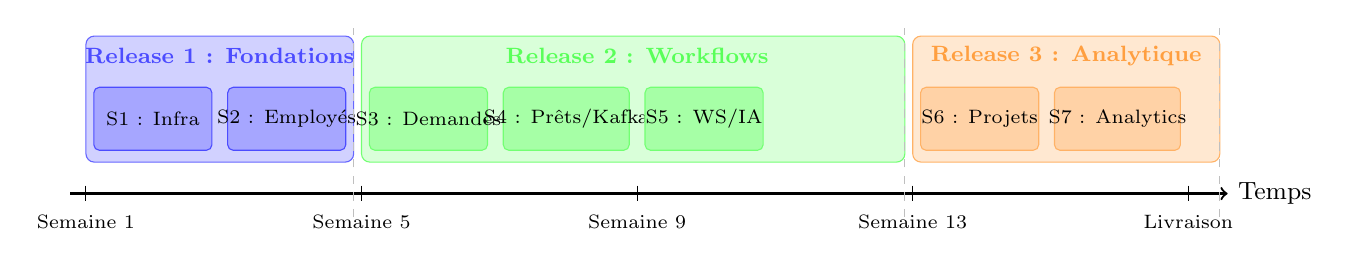
\begin{tikzpicture}[xscale=1.0]

  % Axe temporel
  \draw[thick,->] (-0.2,0) -- (14.5,0) node[right,font=\small]{Temps};
  \foreach \x/\lbl in {0/Semaine 1, 3.5/Semaine 5, 7/Semaine 9, 10.5/Semaine 13, 14/Livraison}{
    \draw (\x,0.1)--(\x,-0.1);
    \node[below,font=\scriptsize] at (\x,-0.15) {\lbl};
  }

  % Release 1 — bleu
  \filldraw[fill=blue!18, draw=blue!60, rounded corners=3pt]
    (0,0.4) rectangle (3.4,2.0);
  \node[font=\footnotesize\bfseries, blue!70] at (1.7,1.75) {Release 1~: Fondations};
  \filldraw[fill=blue!35, draw=blue!70, rounded corners=2pt]
    (0.1,0.55) rectangle (1.6,1.35)
    node[midway,font=\scriptsize]{S1~: Infra};
  \filldraw[fill=blue!35, draw=blue!70, rounded corners=2pt]
    (1.8,0.55) rectangle (3.3,1.35)
    node[midway,font=\scriptsize]{S2~: Employés};

  % Release 2 — vert
  \filldraw[fill=green!15, draw=green!55, rounded corners=3pt]
    (3.5,0.4) rectangle (10.4,2.0);
  \node[font=\footnotesize\bfseries, green!65] at (7.0,1.75) {Release 2~: Workflows};
  \filldraw[fill=green!35, draw=green!55, rounded corners=2pt]
    (3.6,0.55) rectangle (5.1,1.35)
    node[midway,font=\scriptsize]{S3~: Demandes};
  \filldraw[fill=green!35, draw=green!55, rounded corners=2pt]
    (5.3,0.55) rectangle (6.9,1.35)
    node[midway,font=\scriptsize]{S4~: Prêts/Kafka};
  \filldraw[fill=green!35, draw=green!55, rounded corners=2pt]
    (7.1,0.55) rectangle (8.6,1.35)
    node[midway,font=\scriptsize]{S5~: WS/IA};

  % Release 3 — orange
  \filldraw[fill=orange!18, draw=orange!60, rounded corners=3pt]
    (10.5,0.4) rectangle (14.4,2.0);
  \node[font=\footnotesize\bfseries, orange!75] at (12.45,1.75) {Release 3~: Analytique};
  \filldraw[fill=orange!35, draw=orange!60, rounded corners=2pt]
    (10.6,0.55) rectangle (12.1,1.35)
    node[midway,font=\scriptsize]{S6~: Projets};
  \filldraw[fill=orange!35, draw=orange!60, rounded corners=2pt]
    (12.3,0.55) rectangle (13.9,1.35)
    node[midway,font=\scriptsize]{S7~: Analytics};

  % Jalons verticaux
  \foreach \x in {3.4, 10.4, 14.4}
    \draw[dashed,gray!50] (\x,-0.3)--(\x,2.1);

\end{tikzpicture}
\caption{Feuille de route~: 3 releases, 7 sprints, 4 mois}
\label{fig:roadmap}
\end{figure}

\begin{table}[H]
\centering
\caption{Détail des sprints et objectifs}
\label{tab:sprints}
\begin{tabularx}{\textwidth}{|C|l|L|C|}
\hline
\rowcolor{headerblue!25}\textbf{Release} & \textbf{Sprint} & \textbf{Objectif} & \textbf{Durée} \\\hline
\rowcolor{rowgray}
\multirow{2}{*}{R1} & S1 & Infrastructure~: Keycloak, Oracle 23ai, Flyway V1–V4, Angular, Docker & 2 sem. \\\cline{2-4}
& S2 & \textit{employe-service}~: CRUD, code \texttt{EMP-NNNN}, sync Keycloak & 2 sem. \\\hline
\rowcolor{rowgray}
\multirow{3}{*}{R2} & S3 & \textit{demandes-service}~: congés, formations, documents, autorisations & 2 sem. \\\cline{2-4}
& S4 & Prêts, commission de crédit, Apache Kafka, \textit{notification-service} & 2 sem. \\\cline{2-4}
\rowcolor{rowgray}
& S5 & WebSocket STOMP/SockJS, assistant IA Groq (\textit{llama-3.3-70b-versatile}) & 2 sem. \\\hline
\multirow{2}{*}{R3} & S6 & \textit{projets-service}, \textit{taches-service}, recrutement, scoring CV & 2 sem. \\\cline{2-4}
\rowcolor{rowgray}
& S7 & JasperReports (7 templates), analytique, module d'attrition & 2 sem. \\\hline
\end{tabularx}
\end{table}

% ─────────────────────────────────────────────────────────────
\section{Méthodologie de développement~: Scrum}
% ─────────────────────────────────────────────────────────────

\subsection{Comparaison approche classique vs agile}

\begin{table}[H]
\centering
\caption{Comparaison méthode classique~/ méthode agile~: critères de choix pour GerAI}
\label{tab:methodo}
\begin{tabularx}{\textwidth}{|l|L|L|}
\hline
\rowcolor{headerblue!25}\textbf{Critère} &
  \textbf{Cycle en V (classique)} & \textbf{Scrum (agile)} \\\hline
\rowcolor{rowgray}
Périmètre & Figé en amont~; toute évolution est coûteuse &
  Évolutif~; le backlog est reclassifié à chaque sprint \\\hline
Livraison & Un seul livrable en fin de projet &
  Incrément fonctionnel livrable à chaque sprint \\\hline
\rowcolor{rowgray}
Retour client & En début (cahier des charges) et en fin (recette) &
  Continu~; le Product Owner valide chaque incrément \\\hline
Gestion des risques & Risques détectés en phase de test &
  Risques détectés dès la première revue \\\hline
\rowcolor{rowgray}
Convient à GerAI~? &
  \textbf{Non}~: besoins non stabilisés sur 4 modules &
  \textbf{Oui}~: livraisons bi-mensuelles vérifiées \\\hline
\end{tabularx}
\end{table}

\subsection{Cadre Scrum retenu}

Scrum est un cadre de travail itératif fondé sur trois piliers~:
\textbf{transparence} (état réel du travail visible de tous),
\textbf{inspection} (revue régulière de l'incrément) et
\textbf{adaptation} (ajustement du plan en conséquence). Quatre cérémonies
structurent chaque sprint~:

\begin{itemize}
  \item \textbf{Sprint Planning}~: sélection des items du backlog, définition
        du \textit{sprint goal}, décomposition en tâches estimées en points.
  \item \textbf{Daily Standup}~: point quotidien de 15 minutes~: réalisations,
        objectifs du jour, obstacles.
  \item \textbf{Sprint Review}~: démonstration de l'incrément aux parties
        prenantes~; validation fonctionnelle et collecte des retours.
  \item \textbf{Sprint Retrospective}~: analyse du processus~; identification
        d'un point d'amélioration concret pour le sprint suivant.
\end{itemize}

\subsection{Rôles Scrum}

\begin{table}[H]
\centering
\caption{Équipe Scrum du projet GerAI}
\label{tab:scrum_team}
\begin{tabularx}{\textwidth}{|l|l|L|}
\hline
\rowcolor{headerblue!25}\textbf{Rôle} & \textbf{Titulaire} & \textbf{Responsabilités} \\\hline
\rowcolor{rowgray}
Product Owner & Encadrant entreprise & Définit et priorise le Product Backlog selon
  les besoins opérationnels d'Arabsoft~; arbitre les conflits de priorité \\\hline
Scrum Master & Encadrant académique & Facilite les cérémonies~; lève les obstacles
  organisationnels~; veille au respect du cadre \\\hline
\rowcolor{rowgray}
Développeuse & Étudiante & Conçoit, développe, teste et documente l'ensemble
  des incréments~; maintient le backlog technique à jour \\\hline
\end{tabularx}
\end{table}

\subsection{Product Backlog~: extrait priorisé}

\begin{table}[H]
\centering
\caption{Extrait du Product Backlog GerAI}
\label{tab:backlog}
\begin{tabularx}{\textwidth}{|C|l|L|l|C|}
\hline
\rowcolor{headerblue!25}\textbf{ID} & \textbf{Rôle} & \textbf{User Story} & \textbf{Priorité} & \textbf{Sprint} \\\hline
\rowcolor{rowgray}
US-01 & ADMIN\_RH & En tant qu'admin, je veux créer un employé avec génération du code \texttt{EMP-NNNN} et provisioning Keycloak automatique & Haute & 2 \\\hline
US-02 & EMPLOYE & En tant qu'employé, je veux déposer une demande de congé et suivre son état sans relancer le RH & Haute & 3 \\\hline
\rowcolor{rowgray}
US-03 & CHEF & En tant que chef, je veux approuver ou rejeter les demandes de mon équipe avec un commentaire conservé en base & Haute & 3 \\\hline
US-04 & EMPLOYE & En tant qu'employé, je veux connaître ma capacité d'endettement lors du dépôt d'une demande de prêt & Haute & 4 \\\hline
\rowcolor{rowgray}
US-05 & COMITE & En tant que membre de la commission, je veux voter FAVORABLE/DÉFAVORABLE avec suggestion de montant et tranches & Haute & 4 \\\hline
US-06 & EMPLOYE & En tant qu'employé, je veux interroger l'assistant IA sur mes congés et soumettre des demandes par le chat & Moyenne & 5 \\\hline
\rowcolor{rowgray}
US-07 & CHEF & En tant que chef, je veux suivre l'avancement des projets et affecter des tâches aux membres & Haute & 6 \\\hline
US-08 & ADMIN\_RH & En tant qu'admin, je veux consulter le score d'attrition de chaque employé avec le détail des facteurs & Moyenne & 7 \\\hline
\end{tabularx}
\end{table}

\subsection{Organisation d'un sprint}

\begin{figure}[H]
\centering
\begin{tikzpicture}[
  phase/.style={draw, rounded corners=4pt, fill=umlblue!30, minimum width=2.8cm,
                minimum height=1.1cm, font=\small, align=center},
  arr/.style={->, >=stealth, thick}
]
  \node[phase] (pl) at (0,   0) {Sprint\\Planning};
  \node[phase] (dv) at (4.2, 0) {Développement\\10 jours ouvrés};
  \node[phase] (rv) at (8.4, 0) {Sprint\\Review};
  \node[phase] (rp) at (12.6,0) {Rétrospective};

  \node[draw, rounded corners=3pt, fill=orange!25, minimum width=2.5cm,
        minimum height=0.7cm, font=\scriptsize, align=center] (ds) at (4.2,-2)
    {Daily Standup\\(quotidien, 15\,min)};

  \draw[arr] (pl)--(dv) node[midway,above,font=\scriptsize]{Sprint Backlog};
  \draw[arr] (dv)--(rv) node[midway,above,font=\scriptsize]{Incrément};
  \draw[arr] (rv)--(rp);
  \draw[arr,dashed,orange!60] (dv.south)--(ds.north);
  \draw[arr,gray!50] (rp.east) to[bend left=50]
    node[above,font=\scriptsize,gray]{Sprint $n+1$} ++(1.2,0.5);

  \node[font=\scriptsize,gray] at (-2.2,0) {Product\\\textit{Backlog}};
  \draw[arr,gray!50] (-1.5,0)--(-1.3,0);
  \node[font=\scriptsize,gray] at (15,0) {Livrable\\\textit{potentiel}};
  \draw[arr,gray!50] (13.9,0)--(14.1,0);
\end{tikzpicture}
\caption{Cycle d'un sprint Scrum~: cérémonies et livrables}
\label{fig:sprint_cycle}
\end{figure}

% ─────────────────────────────────────────────────────────────
\section{Conclusion}
% ─────────────────────────────────────────────────────────────

Ce chapitre a établi l'ensemble du cadre du projet~: Arabsoft, ses trois
orientations stratégiques et ses insuffisances RH héritées d'une organisation
sans SIRH centralisé~; une analyse comparative qui démontre qu'aucune solution
commerciale ne répond simultanément aux contraintes de coût, de personnalisation
et d'analytique propres à l'entreprise~; une problématique en six exigences~;
la plateforme GerAI comme réponse architecturale~; et Scrum comme cadre de
développement incrémental. Le chapitre suivant détaille la conception, l'architecture
microservices et les choix technologiques qui concrétisent cette vision.
